% Created 2020-02-28 Fri 17:08
% Intended LaTeX compiler: pdflatex
\documentclass[a4paper]{article}

\usepackage{booktabs}
\usepackage[margin=2cm]{geometry}
\usepackage{sourcecodepro}
\usepackage{booktabs}
\usepackage{array}
\usepackage{colortbl}
\usepackage{listings}
\usepackage{algpseudocode}
\usepackage{algorithm}
\usepackage{graphicx}
\usepackage[english]{babel}
\usepackage[scale=2]{ccicons}
\usepackage{hyperref}
\usepackage{relsize}
\usepackage{amsmath}
\usepackage{bm}
\usepackage{amsfonts}
\usepackage{wasysym}
\usepackage{float}
\usepackage{ragged2e}
\usepackage{textcomp}
\usepackage{pgfplots}
\usepackage{todonotes}
\usepgfplotslibrary{dateplot}
\lstdefinelanguage{Julia}%
{morekeywords={abstract,struct,break,case,catch,const,continue,do,else,elseif,%
end,export,false,for,function,immutable,mutable,using,import,importall,if,in,%
macro,module,quote,return,switch,true,try,catch,type,typealias,%
while,<:,+,-,::,/},%
sensitive=true,%
alsoother={$},%
morecomment=[l]\#,%
morecomment=[n]{\#=}{=\#},%
morestring=[s]{"}{"},%
morestring=[m]{'}{'},%
}[keywords,comments,strings]%
\lstset{ %
backgroundcolor={},
basicstyle=\ttfamily\scriptsize,
breakatwhitespace=true,
breaklines=true,
captionpos=n,
extendedchars=true,
frame=n,
language=R,
rulecolor=\color{black},
showspaces=false,
showstringspaces=false,
showtabs=false,
stepnumber=2,
stringstyle=\color{gray},
tabsize=2,
}
\renewcommand*{\UrlFont}{\ttfamily\smaller\relax}
\author{Pedro Bruel}
\date{\today}
\title{Simple Initial Experiment}
\hypersetup{
 pdfauthor={Pedro Bruel},
 pdftitle={Simple Initial Experiment},
 pdfkeywords={},
 pdfsubject={},
 pdfcreator={Emacs 26.3 (Org mode 9.2.5)},
 pdflang={English}}
\begin{document}

\maketitle
The experiment  consists of changing  injection rates  \(inj_1\) and \(inj_2\),  for 2
applications in  Supersim, and optimize the  execution times \(\mathcal{P}(inj_1)\)
and \(\mathcal{P}(inj_2)\).  The experimental settings are:

\begin{center}
\begin{tabular}{ll}
\hline
Parameter & Value\\
\hline
Injection Rate 1 (\(inj_1\)) & \([0.1, 0.5]\)\\
Injection Rate 2 (\(inj_2\)) & \([0.1, 0.5]\)\\
Performance Metric & \(\frac{\mathcal{P}_1(inj_1) + \mathcal{P}_2(inj_2)}{2}\)\\
\hline
\end{tabular}
\end{center}

The interval for  injection rates was limited because the  simulator crashed for
larger rates.   The problem must  be better  understood to determine  the proper
injection rate ranges.

Low-discrepancy samples  of size 20 were  taken for both injection  rates on the
specified intervals,  and 10 repetitions  were performed. In total,  200 samples
were measured, and the best value according to the performance metric was logged
separately for each repetition.

The figure  below shows the injection  rates, for both applications,  in the 200
samples tested.

\begin{center}
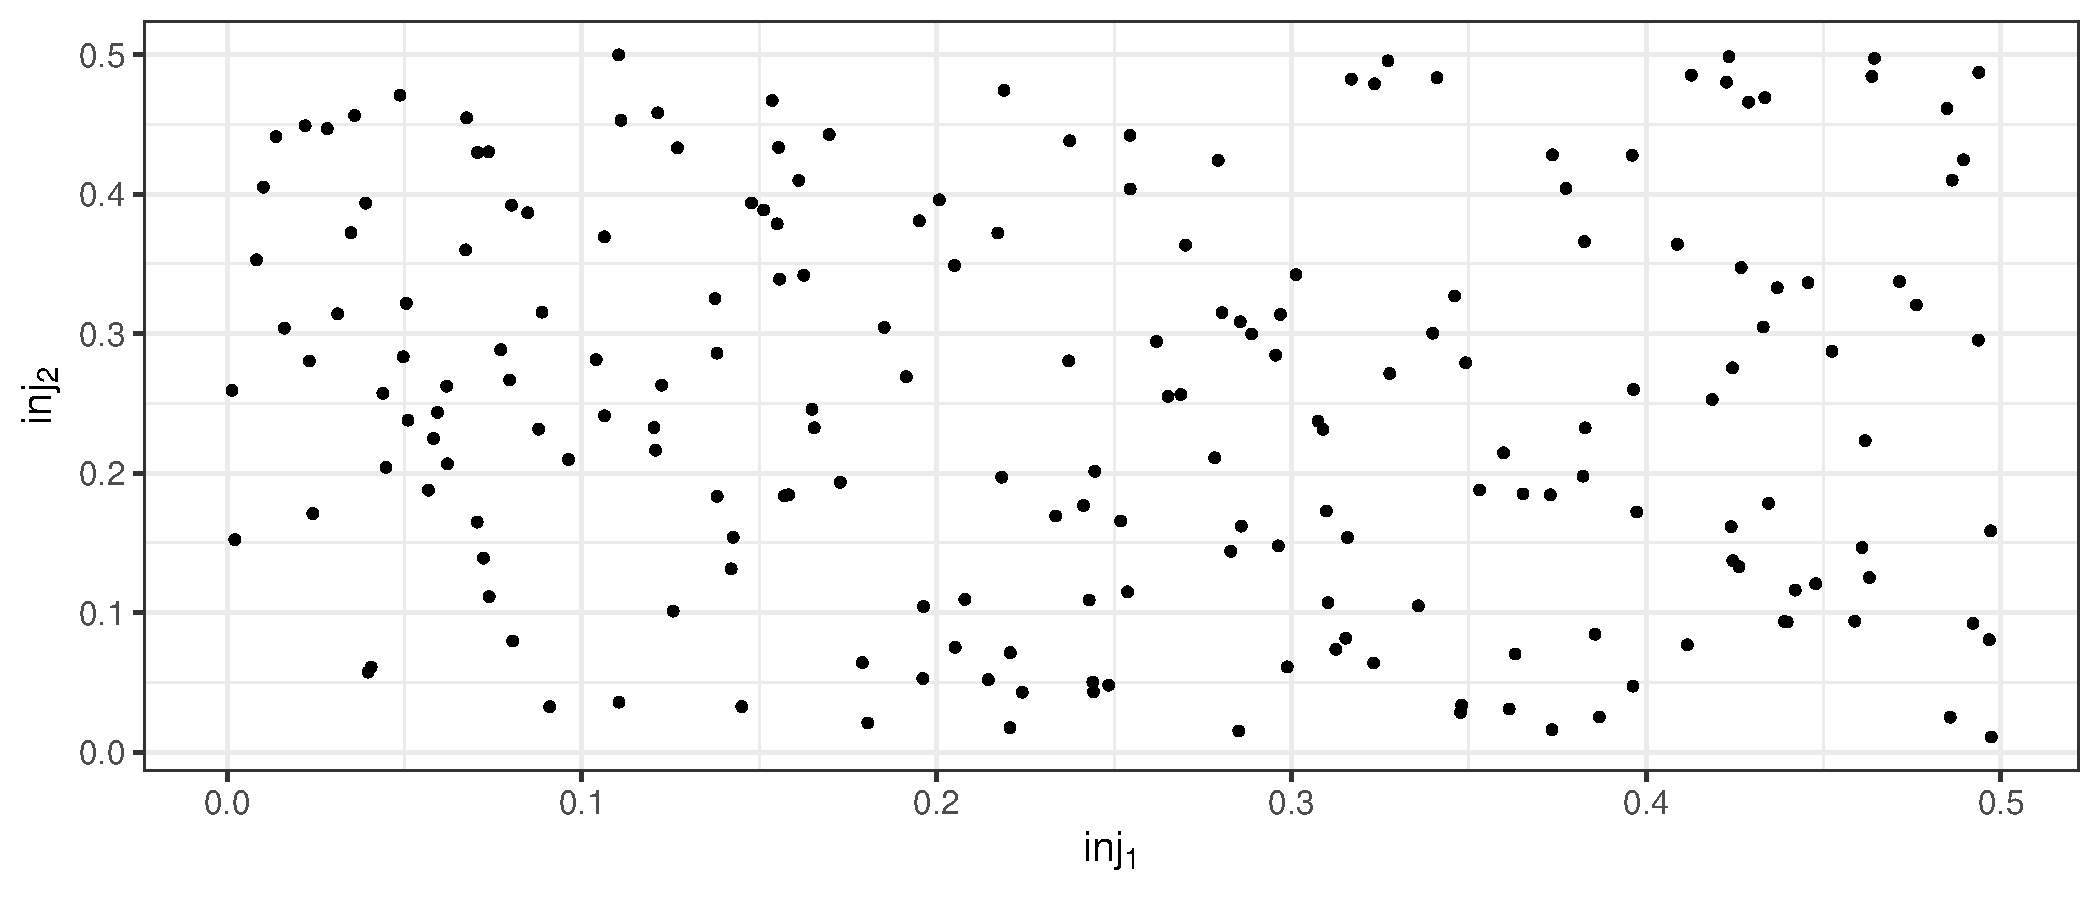
\includegraphics[width=0.4\textwidth]{./img/2_apps_min_mean_time/rs_20_samples_10_iterations_injection_scatter.pdf}
\end{center}

\section{Initial Results}
\label{sec:org6afd1e3}
\subsection{Histograms}
\label{sec:org7050a16}
Looking at the  histograms of the performance metric and  the execution times of
both  applications,  in  the  figure  below,  we see  that  almost  150  of  the
configurations tested had performance below \(10^{9}\).

\begin{center}
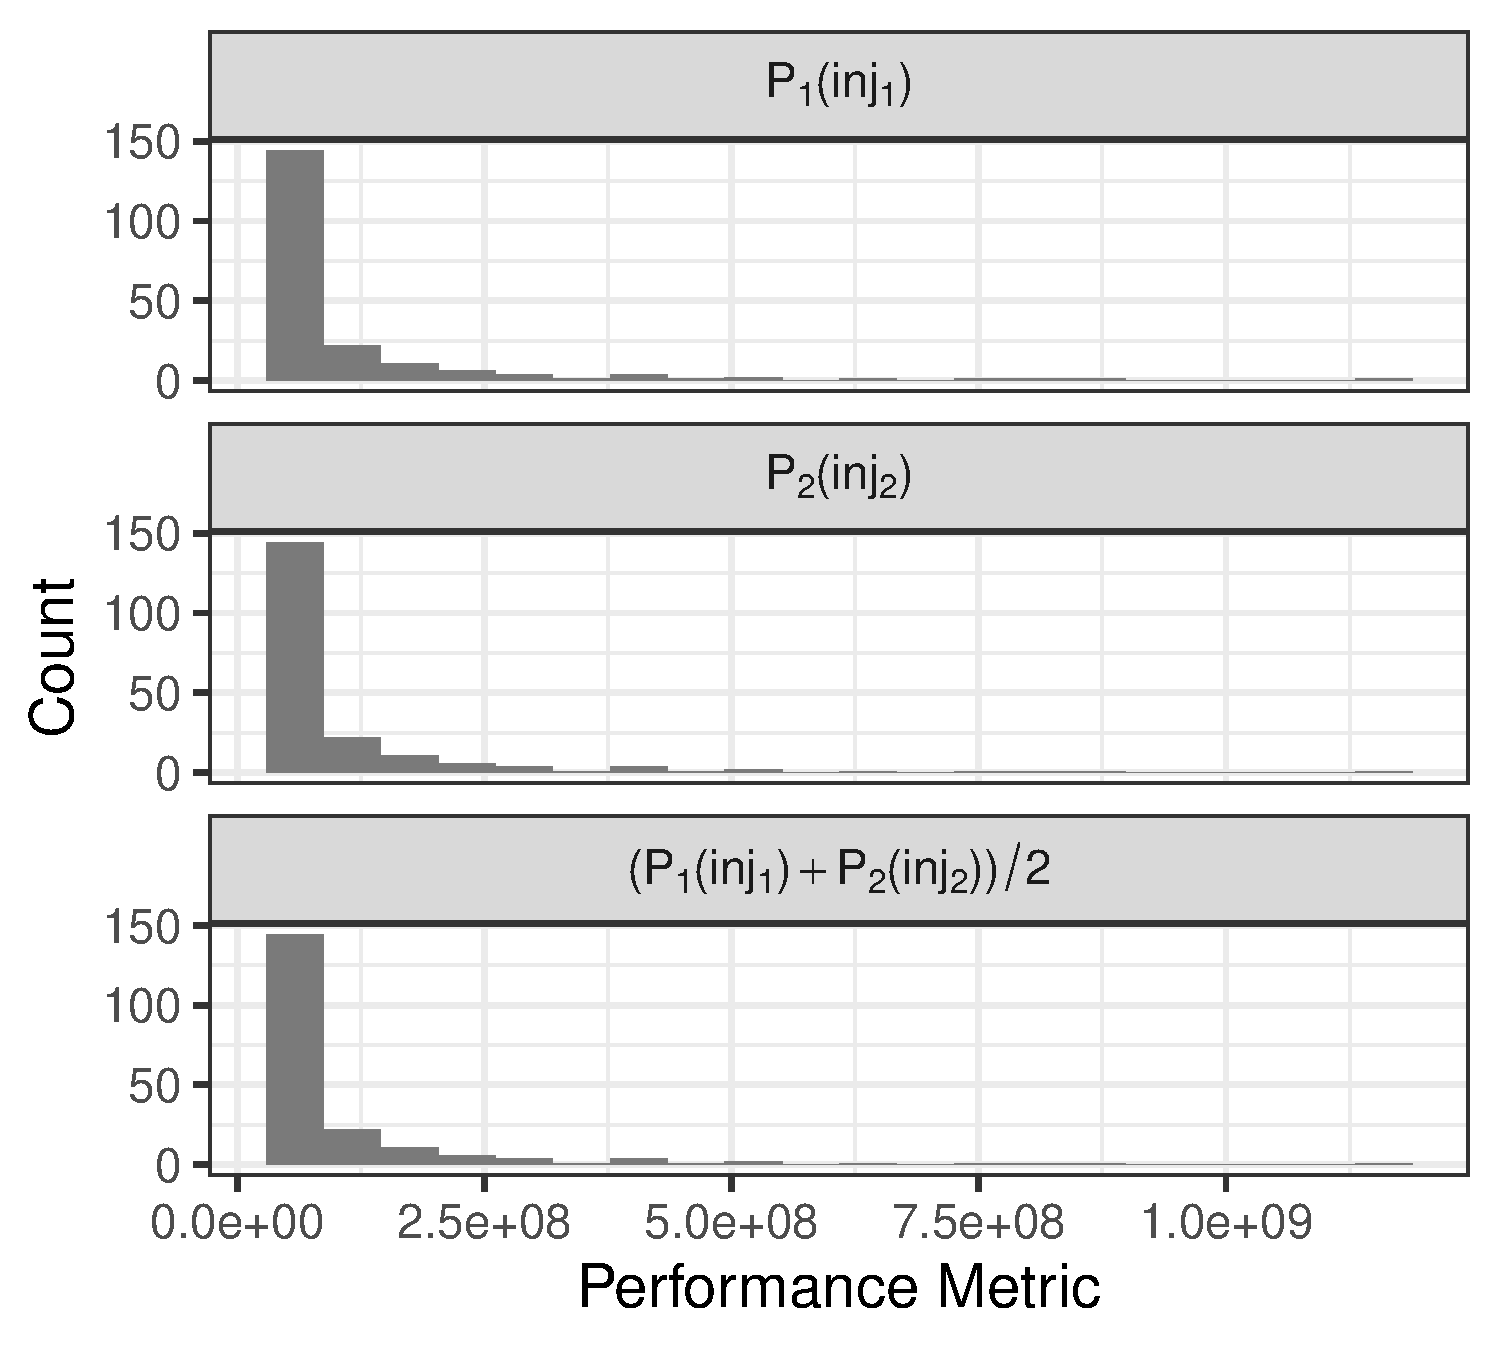
\includegraphics[width=0.5\textwidth]{./img/2_apps_min_mean_time/rs_20_samples_10_iterations_histogram.pdf}
\end{center}

Below, we take a closer look at the lower end performance measurements.

\begin{center}
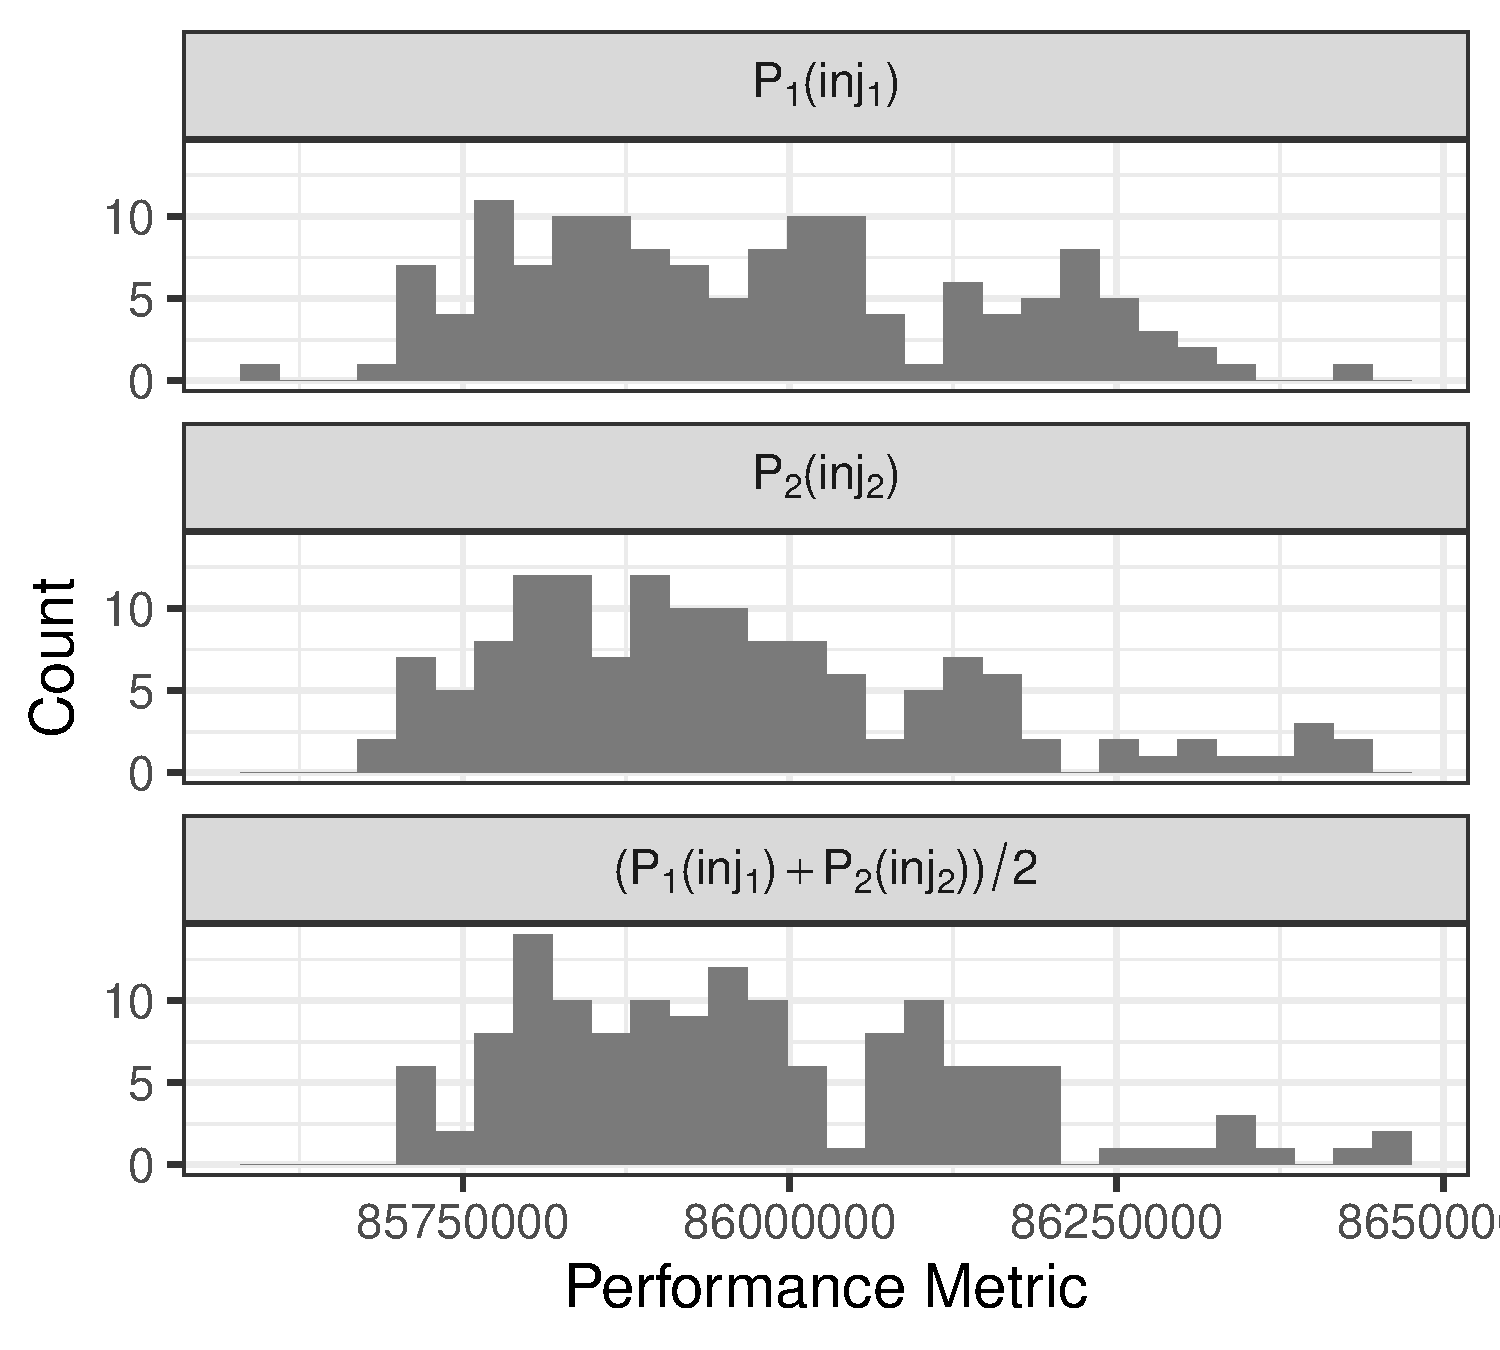
\includegraphics[width=0.5\textwidth]{./img/2_apps_min_mean_time/rs_20_samples_10_iterations_histogram_cut.pdf}
\end{center}

\subsection{Performance Metric and Injection Rate}
\label{sec:orge7d9b4d}
We  now  look  at  the  performance metric  measured  for  each  injection  rate
configuration.  The  figure below splits the  values of injection rate  for each
application, and shows the performance metric computed using the execution times
of both applications.

\begin{center}
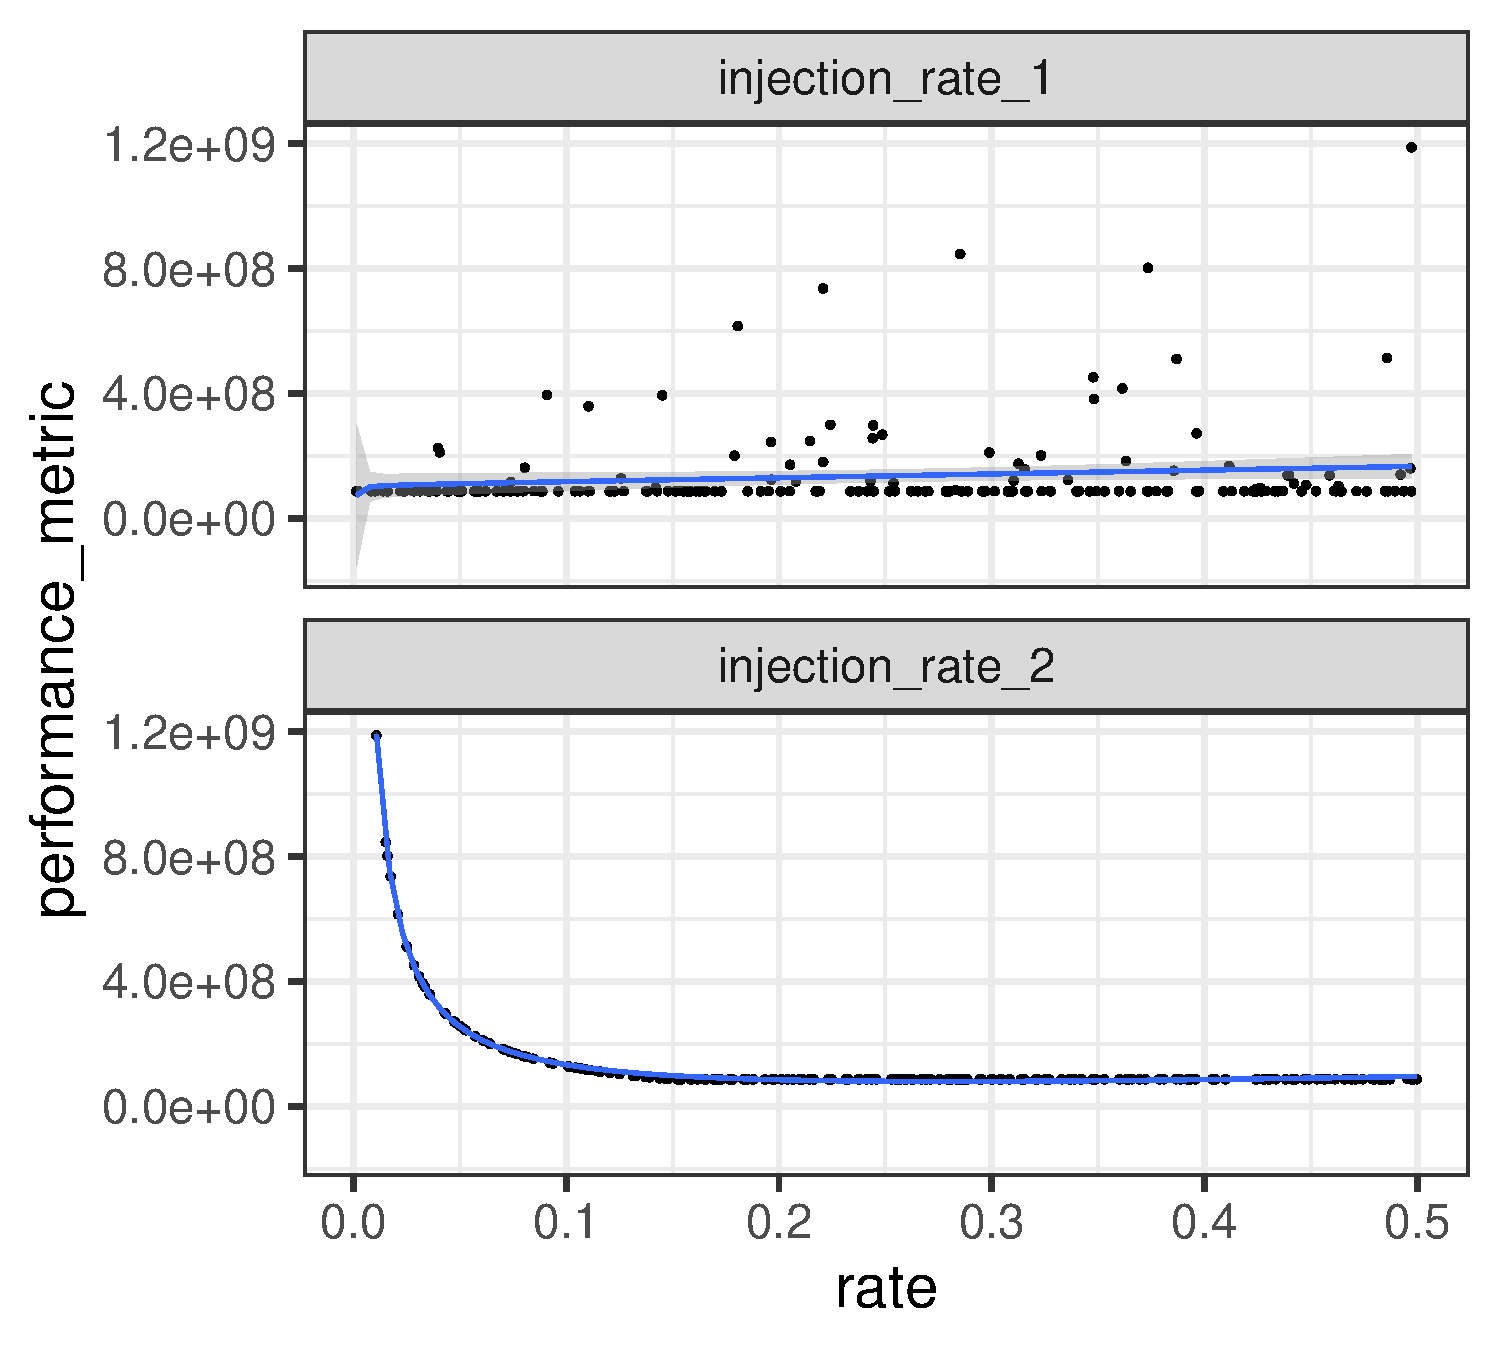
\includegraphics[width=0.6\textwidth]{./img/2_apps_min_mean_time/rs_20_samples_10_iterations_scatter.pdf}
\end{center}

\subsection{ANOVA and Goodness of Fit}
\label{sec:orgcfaeec5}
% latex table generated in R 3.6.2 by xtable 1.8-4 package
% Fri Feb 28 17:07:50 2020
\begin{table}[ht]
\centering
\begin{tabular}{lr}
  \toprule
Model Term & Significance p-value \\
  \midrule
(Intercept & $2.3 \times 10^{-6}$ \\
  injection\_rate\_1 & $1.9 \times 10^{-2}$ \\
  injection\_rate\_2 & $3.8 \times 10^{-63}$ \\
  1/injection\_rate\_1 & $1.8 \times 10^{-2}$ \\
  1/injection\_rate\_2 & $8.4 \times 10^{-261}$ \\
  1/injection\_rate\_1$\times$1/injection\_rate\_2 & $8.5 \times 10^{-3}$ \\
   \bottomrule
\end{tabular}
\end{table}

% latex table generated in R 3.6.2 by xtable 1.8-4 package
% Fri Feb 28 17:07:42 2020
\begin{table}[ht]
\centering
\begin{tabular}{lr}
  \toprule
Model Term & Significance p-value \\
  \midrule
injection\_rate\_1 & $4.3 \times 10^{-115}$ \\
  injection\_rate\_2 & $2.2 \times 10^{-225}$ \\
  1/injection\_rate\_1 & $7.2 \times 10^{-19}$ \\
  1/injection\_rate\_2 & $6.9 \times 10^{-267}$ \\
  1/injection\_rate\_1$\times$1/injection\_rate\_2 & $8.5 \times 10^{-3}$ \\
   \bottomrule
\end{tabular}
\end{table}
\end{document}
